\documentclass[12pt, a4paper]{book}

\usepackage[T1]{fontenc}
\usepackage[utf8]{inputenc}
\usepackage[charter, cal=cmcal]{mathdesign}
\usepackage[scaled=0.92]{helvet}
\usepackage{geometry}
\geometry{a4paper, top=30mm, bottom=30mm, inner=32mm, outer=25mm, marginparwidth=18mm}

\usepackage{amsmath, amsthm}
\usepackage[version=4]{mhchem}
\usepackage{graphicx}
\usepackage{xcolor}
\usepackage{tikz}
\usetikzlibrary{arrows.meta, shapes.geometric, positioning, calc, backgrounds}
\usepackage{pgfplots}
\pgfplotsset{compat=1.18}
\usepackage{tcolorbox}
\tcbuselibrary{skins, breakable, theorems}
\usepackage{titlesec}
\usepackage{fancyhdr}
\usepackage{enumitem}
\usepackage{booktabs}
\usepackage{array}
\usepackage{parskip}
\usepackage{siunitx}
\usepackage[colorlinks=true, linkcolor=BrickRed,
            urlcolor=NavyBlue, citecolor=ForestGreen]{hyperref}

% ── Colours (Charcoal / Royal Blue) ──────────────────────────────────────────
\definecolor{JourneyColor}{HTML}{0F172A}
\definecolor{ModuleColor}{HTML}{2563EB}
\definecolor{PuzzleColor}{HTML}{D97706}
\definecolor{DiscoveryColor}{HTML}{3B82F6}
\definecolor{WarningColor}{HTML}{991B1B}
\definecolor{ProblemColor}{HTML}{6B21A8}
\definecolor{ReflectColor}{HTML}{0D9488}
\definecolor{HistoryColor}{HTML}{78350F}

% ── Boxes ─────────────────────────────────────────────────────────────────────
\newtcolorbox{puzzlebox}[1][]{enhanced,breakable,
  colback=PuzzleColor!6,colframe=PuzzleColor,fonttitle=\bfseries\sffamily,
  title={The Puzzle},attach boxed title to top left={yshift=-2mm,xshift=6mm},
  boxed title style={colback=PuzzleColor},borderline west={3pt}{0pt}{PuzzleColor},#1}

\newtcolorbox{discoverybox}[1][]{enhanced,breakable,
  colback=DiscoveryColor!8,colframe=DiscoveryColor,fonttitle=\bfseries\sffamily,
  title={Discovery},attach boxed title to top left={yshift=-2mm,xshift=6mm},
  boxed title style={colback=DiscoveryColor},borderline west={3pt}{0pt}{DiscoveryColor},#1}

\newtcolorbox{problembox}[1][]{enhanced,breakable,
  colback=ProblemColor!5,colframe=ProblemColor,fonttitle=\bfseries\sffamily,
  title={Problems},attach boxed title to top left={yshift=-2mm,xshift=6mm},
  boxed title style={colback=ProblemColor},borderline west={3pt}{0pt}{ProblemColor},#1}

\newtcolorbox{deepbox}[1][]{enhanced,breakable,
  colback=JourneyColor!5,colframe=JourneyColor,fonttitle=\bfseries\sffamily,
  title={Deep Problems},attach boxed title to top left={yshift=-2mm,xshift=6mm},
  boxed title style={colback=JourneyColor},borderline west={4pt}{0pt}{JourneyColor},#1}

\newtcolorbox{historybox}[1][]{enhanced,breakable,
  colback=HistoryColor!7,colframe=HistoryColor!60,fonttitle=\bfseries\sffamily\small,
  title={Historical Note},attach boxed title to top left={yshift=-2mm,xshift=6mm},
  boxed title style={colback=HistoryColor!80},#1}

\newtcolorbox{reflectionbox}[1][]{enhanced,breakable,
  colback=ReflectColor!6,colframe=ReflectColor,fonttitle=\bfseries\sffamily,
  title={Reflection},attach boxed title to top left={yshift=-2mm,xshift=6mm},
  boxed title style={colback=ReflectColor},borderline west={3pt}{0pt}{ReflectColor},#1}

\newtcolorbox{namedconcept}[2][]{enhanced,
  colback=ModuleColor!6,colframe=ModuleColor,fonttitle=\bfseries\sffamily\large,
  title={#2},attach boxed title to top left={yshift=-2mm,xshift=6mm},
  boxed title style={colback=ModuleColor},#1}

% ── Section formatting ────────────────────────────────────────────────────────
\titleformat{\chapter}[display]
  {\normalfont\sffamily\huge\bfseries\color{JourneyColor}}
  {\textcolor{JourneyColor!60}{\chaptertitlename\ \thechapter}}{10pt}{\Huge}
  [\vspace{2pt}\textcolor{JourneyColor}{\titlerule[1.5pt]}]
\titleformat{\section}
  {\normalfont\sffamily\Large\bfseries\color{ModuleColor}}
  {\thesection}{1em}{}[\textcolor{ModuleColor!40}{\titlerule[0.6pt]}]
\titleformat{\subsection}
  {\normalfont\sffamily\large\bfseries\color{JourneyColor!80}}{\thesubsection}{1em}{}
\titleformat{\subsubsection}
  {\normalfont\sffamily\normalsize\bfseries}{\thesubsubsection}{1em}{}

\pagestyle{fancy}
\fancyhf{}
\fancyhead[LE]{\small\sffamily\textcolor{JourneyColor}{\leftmark}}
\fancyhead[RO]{\small\sffamily\textcolor{ModuleColor}{\rightmark}}
\fancyfoot[C]{\small\thepage}
\renewcommand{\headrulewidth}{0.4pt}

\newcommand{\newterm}[1]{\textit{\textcolor{DiscoveryColor}{#1}}}
\newcommand{\important}[1]{\textcolor{ModuleColor}{\textbf{#1}}}

\begin{document}

\setcounter{chapter}{3}
\chapter[Journey 4 --- Programming Paradigms and Language Semantics]
        {Journey Four\\[8pt]
         \textcolor{ModuleColor}{\large Programming Paradigms and Language Semantics}}
\setcounter{section}{0}

\section{Module 4.1 --- Lambda Calculus and Functional Computation}
\label{sec:mod4.1}

\subsection*{Motivation}

We completed in Journey 3 the abstract limits of decidability, studying what Turing Machines can calculate.
But knowing a machine exists is not the same as writing code.
To build software, we must design languages that bridge human thought and physical execution.

We begin our study of language semantics with Alonzo Church's **Lambda Calculus ($\lambda$-calculus)**.
Invented in the 1930s (simultaneously with Turing's work), the $\lambda$-calculus is the ultimate minimalist programming language.
It has no primitive data: no numbers, no booleans, and no memory states. It contains only variables, function definitions, and function applications.
Yet, this simple system is Turing-complete.
This module formalizes the syntax and reductions of the untyped $\lambda$-calculus, shows how to compile numbers and logic using pure functions (Church Encodings), and derives the **Y Combinator** that unlocks recursion.

\subsection{Computation Without Data}

We examine how to construct a Turing-complete system using only function application.

\begin{puzzlebox}
\textbf{The Stateless Language.}

Suppose we want to design a programming language, but we are forbidden from using *any* primitive data.
We have no numbers ($0, 1, 2$), no booleans ($\text{true, false}$), and no memory registers.
Our only tool is the ability to define functions, bind variables, and apply functions to other functions.
\begin{enumerate}[label=(\alph*), leftmargin=*]
  \item We define a Boolean as a function of two arguments that selects one of them:
        * $\text{true} \equiv \lambda x. \lambda y. x$ (returns the first argument).
        * $\text{false} \equiv \lambda x. \lambda y. y$ (returns the second argument).
        Using these definitions, show that the conditional statement `if-then-else` is simply function application: $\text{if } b \text{ then } t \text{ else } e \equiv b \, t \, e$.
        (Evaluate $b \, t \, e$ when $b = \text{true}$ and when $b = \text{false}$).
  \item We represent a number $n$ (a **Church Numeral**) as a function that applies a function $f$ to an argument $x$ exactly $n$ times:
        * $c_0 \equiv \lambda f. \lambda x. x$
        * $c_1 \equiv \lambda f. \lambda x. f \, x$
        * $c_2 \equiv \lambda f. \lambda x. f (f \, x)$
        We define the **Successor** function $\text{succ}$ (which computes $n+1$) as:
        \[
          \text{succ} \;\equiv\; \lambda n. \lambda f. \lambda x. f (n \, f \, x).
        \]
        Evaluate $\text{succ} \, c_1$ step-by-step using variable substitution. Show that it reduces to $c_2$.
  \item Because functions are anonymous in this calculus, we cannot write recursive functions by referencing their name (e.g. we cannot write $f = \dots f \dots$).
        How do we perform recursion if we cannot name our functions?
\end{enumerate}
\end{puzzlebox}

\subsection{Syntax and Reductions}

We formalize the mathematical rules of the untyped lambda calculus.

\begin{namedconcept}{Lambda Calculus Syntax}
The terms of the untyped $\lambda$-calculus are defined by the context-free grammar:
\[
  e \;::=\; x \;\mid\; \lambda x. e \;\mid\; e_1 \, e_2
\]
where:
1. $x$ is a **Variable**.
2. $\lambda x. e$ is an **Abstraction** (defining an anonymous function with parameter $x$ and body $e$).
3. $e_1 \, e_2$ is an **Application** (applying function $e_1$ to argument $e_2$).
\end{namedconcept}

\begin{explobox}
Computation in the $\lambda$-calculus is driven by two substitution rules:
* **$\alpha$-conversion (Renaming):** $\lambda x. x \equiv_\alpha \lambda y. y$. We can rename bound variables to avoid conflicts.
* **$\beta$-reduction (Evaluation):** Applying an abstraction to an argument replaces all free occurrences of the bound variable in the body with the argument:
  \[
    (\lambda x. e_1) \, e_2 \;\to_\beta\; e_1[x \mapsto e_2].
  \]
\begin{enumerate}[label=(\alph*), leftmargin=*]
  \item Identify the free and bound variables in the term: $(\lambda x. x \, y) \, (\lambda y. y)$.
  \item Evaluate the following term step-by-step using $\beta$-reductions, renaming variables as necessary to avoid capturing:
        \[
          (\lambda x. \lambda y. x \, y) \, (\lambda z. z \, z) \, w.
        \]
  \item A term is in **normal form** if it cannot be reduced further.
        Some terms have no normal form. Evaluate the term:
        \[
          \Omega \;\equiv\; (\lambda x. x \, x) \, (\lambda x. x \, x).
        \]
        What happens when you apply $\beta$-reduction to $\Omega$?
\end{enumerate}
\end{explobox}

\subsection{Recursion and the Y Combinator}

We resolve the problem of anonymous recursion using fixed-point theory.

\begin{explobox}
A **fixed point** of a function $F$ is a value $x$ such that $F \, x = x$.
In the $\lambda$-calculus, we can find the fixed point of any term using a **Fixed-Point Combinator**. The most famous is the **Y Combinator** (discovered by Haskell Curry):
\[
  Y \;\equiv\; \lambda f. (\lambda x. f (x \, x)) \, (\lambda x. f (x \, x)).
\]
\begin{enumerate}[label=(\alph*), leftmargin=*]
  \item Prove that the Y combinator satisfies the fixed-point equation under $\beta$-reduction:
        \[
          Y \, F \;\to_\beta\; F(Y \, F)
        \]
        for any lambda term $F$.
  \item Suppose we want to write a recursive factorial function:
        \[
          \text{fact} \, n \;=\; \text{if } (\text{iszero } n) \text{ then } c_1 \text{ else } (\text{mult } n \, (\text{fact } (\text{pred } n))).
        \]
        We rewrite this by abstracting the recursive call as a parameter $f$:
        \[
          G \;\equiv\; \lambda f. \lambda n. \text{if } (\text{iszero } n) \text{ then } c_1 \text{ else } (\text{mult } n \, (f \, (\text{pred } n))).
        \]
        Explain why defining $\text{fact} \equiv Y \, G$ successfully implements the recursive factorial function. (Show how the first step of evaluation unfolds).
\end{enumerate}
\end{explobox}

\newpage

% ─── Section: Discovery ──────────────────────────────────────────────────────
\section{Part 3 --- Discovery}

\begin{discoverybox}
\textbf{What have we built?}

\textbf{First.} The untyped $\lambda$-calculus is a Turing-complete system built entirely on variable binding (abstraction) and substitution (application).

\textbf{Second.} $\beta$-reduction represents the core step of execution, substituting argument terms for parameters within function bodies.

\textbf{Third.} Church encodings allow us to represent booleans, numbers, and logical operations using pure functions.

\textbf{Fourth.} The Y Combinator is a fixed-point combinator that enables recursion in a language of anonymous functions by continuously duplicating the function body during evaluation.
\end{discoverybox}

\newpage

% ─── Section: Naming Concepts ────────────────────────────────────────────────
\section{Part 4 --- What This Is Called}

\begin{namedconcept}{Functional calculus parameters}
* **$\lambda$-Calculus:** Alonzo Church's formal system for function definition, application, and recursion.
* **Abstraction:** The term $\lambda x. e$, defining a function with parameter $x$.
* **Application:** The term $e_1 \, e_2$, executing a function call.
* **$\beta$-Reduction:** The evaluation step of substituting arguments into function bodies.
* **Church Numeral:** A functional representation of integers, where $n$ is represented by $n$ applications of a function.
* **Y Combinator:** The fixed-point operator used to implement recursion in the untyped $\lambda$-calculus.
\end{namedconcept}

\newpage

% ─── Section: Solved Exercises ───────────────────────────────────────────────
\section{Part 5 --- Solved Exercises}

\begin{problembox}
\begin{enumerate}[label=\textbf{E\arabic*.}]
  \item \textbf{Beta-Reduction Step-by-Step.}
  
        Evaluate the lambda term $(\lambda x. \lambda y. x \, y \, x) \, (\lambda z. z) \, w$ step-by-step using $\beta$-reduction.
        
        \textbf{Solution:}
        The term is:
        \[
          \left( (\lambda x. \lambda y. x \, y \, x) \, (\lambda z. z) \right) \, w.
        \]
        1. **First step:** We apply the leftmost abstraction $\lambda x$ to the argument $(\lambda z. z)$.
           This replaces all occurrences of $x$ in the body $\lambda y. x \, y \, x$ with $(\lambda z. z)$:
           \[
             (\lambda x. \lambda y. x \, y \, x) \, (\lambda z. z) \;\to_\beta\; \lambda y. (\lambda z. z) \, y \, (\lambda z. z).
           \]
        2. **Second step:** Now substitute this back into the full term:
           \[
             \left( \lambda y. (\lambda z. z) \, y \, (\lambda z. z) \right) \, w.
           \]
           We apply the abstraction $\lambda y$ to the argument $w$.
           This replaces $y$ with $w$:
           \[
             (\lambda z. z) \, w \, (\lambda z. z).
           \]
        3. **Third step:** Now we evaluate the application $(\lambda z. z) \, w$.
           We apply the identity function $\lambda z. z$ to the argument $w$:
           \[
             (\lambda z. z) \, w \;\to_\beta\; w.
           \]
           This leaves:
           \[
             w \, (\lambda z. z).
           \]
        Since this term cannot be reduced further, it is in normal form.
        Thus, the final reduced term is $w \, (\lambda z. z)$.
        
  \item \textbf{Church Addition Proof.}
  
        We define the Church addition function as:
        \[
          \text{add} \;\equiv\; \lambda m. \lambda n. \lambda f. \lambda x. m \, f \, (n \, f \, x).
        \]
        Prove that $\text{add} \, c_1 \, c_1 \to_\beta c_2$.
        
        \textbf{Solution:}
        Recall the Church numerals:
        * $c_1 \equiv \lambda f. \lambda x. f \, x$.
        * $c_2 \equiv \lambda f. \lambda x. f (f \, x)$.
        
        1. **Substitute inputs into addition function:**
           \[
             \text{add} \, c_1 \, c_1 \;\to_\beta\; \left( \lambda m. \lambda n. \lambda f. \lambda x. m \, f \, (n \, f \, x) \right) \, c_1 \, c_1.
           \]
           Apply $m \mapsto c_1$:
           \[
             \left( \lambda n. \lambda f. \lambda x. c_1 \, f \, (n \, f \, x) \right) \, c_1.
           \]
           Apply $n \mapsto c_1$:
           \[
             \lambda f. \lambda x. c_1 \, f \, (c_1 \, f \, x).
           \]
        2. **Evaluate the sub-terms:**
           Recall $c_1 = \lambda f. \lambda x. f \, x$.
           * Evaluate $c_1 \, f \, x$:
             \[
               (\lambda f. \lambda x. f \, x) \, f \, x \;\to_\beta\; (\lambda x. f \, x) \, x \;\to_\beta\; f \, x.
             \]
             So, $c_1 \, f \, x = f \, x$.
           * Now evaluate $c_1 \, f \, (c_1 \, f \, x)$:
             Using the result above, let $y = c_1 \, f \, x = f \, x$.
             \[
               c_1 \, f \, y \;\to_\beta\; f \, y \;=\; f (f \, x).
             \]
        3. **Assemble the final term:**
           Substitute $c_1 \, f \, (c_1 \, f \, x) \to_\beta f (f \, x)$ back into the abstraction:
           \[
             \lambda f. \lambda x. f (f \, x).
           \]
        By definition, this is exactly the Church numeral $c_2$.
        This completes the proof.
\end{enumerate}
\end{problembox}

\newpage

% ─── Section: Problems ───────────────────────────────────────────────────────
\section{Part 6 --- Problems}

\begin{problembox}
\begin{enumerate}[label=\textbf{P\arabic*.}]
  \item \textbf{Church Multiplication and Exponentiation.}
  
        Church Numerals are defined as $c_n \equiv \lambda f. \lambda x. f^n(x)$.
        \begin{enumerate}[label=(\alph*)]
          \item Prove that multiplication is represented by the term:
                \[
                  \text{mult} \;\equiv\; \lambda m. \lambda n. \lambda f. m (n \, f).
                \]
                Show that $\text{mult} \, c_2 \, c_2 \to_\beta c_4$.
          \item Exponentiation (computing $m^n$) is represented by the incredibly simple term:
                \[
                  \text{exp} \;\equiv\; \lambda m. \lambda n. n \, m.
                \]
                Evaluate $\text{exp} \, c_2 \, c_3$ (which computes $2^3 = 8$) and show that it reduces to $c_8$.
                *(Hint: Recall that $c_3 \, F \to F (F (F \, x))$, so $c_3 \, c_2$ applies $c_2$ to itself three times).*
        \end{enumerate}

  \item \textbf{Evaluation Strategies and Infinite Terms.}
  
        A lambda term can contain multiple sub-expressions that can be reduced (called **redexes**). We define two primary evaluation strategies:
        * **Call-by-Name (Normal Order):** Always reduce the leftmost, outermost redex first.
        * **Call-by-Value (Applicative Order):** Reduce the arguments to their normal form before applying the function.
        
        Consider the infinite looping term $\Omega \equiv (\lambda x. x \, x) \, (\lambda x. x \, x)$ and the term:
        \[
          E \;\equiv\; (\lambda y. c_5) \, \Omega.
        \]
        \begin{enumerate}[label=(\alph*)]
          \item Show that $\Omega \to_\beta \Omega$ (beta-reduces to itself in a single step).
          \item Evaluate the term $E$ using **Call-by-Name**. Show that it halts and returns $c_5$.
          \item Evaluate the term $E$ using **Call-by-Value**.
                Why does Call-by-Value fail to halt, entering an infinite loop?
          \item What does this trade-off reveal about the implementation of "lazy evaluation" in languages like Haskell versus "eager evaluation" in languages like C or Python?
        \end{enumerate}
\end{enumerate}
\end{problembox}

\newpage

% ─── Section: Deep Problems ──────────────────────────────────────────────────
\section{Part 7 --- Deep Problems}

\begin{deepbox}
\begin{enumerate}[label=\textbf{D\arabic*.}]
  \item \textbf{The Y Combinator fixed point Proof.}
  
        We prove that the Y combinator correctly acts as a universal fixed-point finder:
        \[
          Y \, F \;\to_\beta\; F (Y \, F).
        \]
        Let $Y \equiv \lambda f. (\lambda x. f (x \, x)) \, (\lambda x. f (x \, x))$.
        
        \begin{enumerate}[label=(\alph*)]
          \item Apply $Y$ to a term $F$. Evaluate the first step of $\beta$-reduction to show:
                \[
                  Y \, F \;\to_\beta\; (\lambda x. F (x \, x)) \, (\lambda x. F (x \, x)).
                \]
          \item Now, look at the right-hand term: $W \equiv (\lambda x. F (x \, x)) \, (\lambda x. F (x \, x))$.
                Evaluate the next step of $\beta$-reduction on $W$ itself, replacing occurrences of $x$ in the body $F(x\,x)$ with the argument $(\lambda x. F (x \, x))$.
                Show that this yields:
                \[
                  W \;\to_\beta\; F \left( (\lambda x. F (x \, x)) \, (\lambda x. F (x \, x)) \right).
                \]
          \item Use this to conclude that $Y \, F \to_\beta F (Y \, F)$.
          \item The Y combinator works in Call-by-Name, but loops infinitely in Call-by-Value.
                To solve this, we define the **Z Combinator** (the call-by-value fixed-point operator):
                \[
                  Z \;\equiv\; \lambda f. (\lambda x. f (\lambda y. x \, x \, y)) \, (\lambda x. f (\lambda y. x \, x \, y)).
                \]
                Explain how the addition of the abstraction $\lambda y$ prevents infinite expansion under eager evaluation.
        \end{enumerate}

  \item \textbf{The Church-Rosser Theorem and Uniqueness of Normal Forms.}
  
        The untyped $\lambda$-calculus is highly flexible, but is it consistent?
        Let $\to_\beta^*$ denote the relation "reduces to in zero or more steps".
        * **The Church-Rosser Theorem (Confluence):** If $a \to_\beta^* b$ and $a \to_\beta^* c$, then there exists a term $d$ such that $b \to_\beta^* d$ and $c \to_\beta^* d$.
        
        \begin{center}
        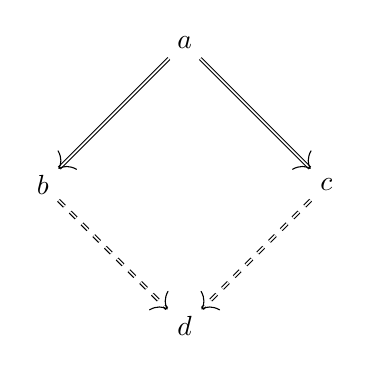
\begin{tikzpicture}[scale=1.2]
          \node (a) at (0,2) {$a$};
          \node (b) at (-1.5,0.5) {$b$};
          \node (c) at (1.5,0.5) {$c$};
          \node (d) at (0,-1) {$d$};
          
          \draw[->, double] (a) -- (b);
          \draw[->, double] (a) -- (c);
          \draw[->, dashed, double] (b) -- (d);
          \draw[->, dashed, double] (c) -- (d);
        \end{tikzpicture}
        \end{center}
        
        \begin{enumerate}[label=(\alph*)]
          \item Prove that if a lambda term has a normal form, this normal form is unique.
                *(Hint: Assume $a$ reduces to two distinct normal forms $b$ and $c$. Apply the Church-Rosser theorem to find $d$. Since $b$ and $c$ are normal forms, what must be true about their transitions to $d$?)*
          \item Explain the physical significance of the Church-Rosser theorem for compilers: why is the final result of compiling and optimizing code independent of the order in which the compiler optimizer chooses to evaluate sub-expressions?
        \end{enumerate}
\end{enumerate}
\end{deepbox}

\newpage

% ─── Section: Reflection ─────────────────────────────────────────────────────
\section{Part 8 --- Reflection}

\begin{reflectionbox}
\textbf{Conceptual Reflection}

Consider the following questions:
\begin{enumerate}
  \item **On the Minimalism of Computation:** The Lambda Calculus uses only three syntactic constructs (variables, abstraction, application). It has no loops, no state, and no data types. Yet it is completely equivalent in power to a Turing Machine. What does this reveal about the nature of computation—is it inherently about states (Turing) or about function substitutions (Church)?
  \item **On the Invention of Data:** In the Lambda Calculus, numbers and booleans are not built-in components, but are invented out of pure behavior (functions). Does this imply that data is ultimately a secondary property, and that all data types are just patterns of action?
  \item **On the Arrow of Evaluation:** We saw that Call-by-Name can evaluate terms that Call-by-Value cannot (by ignoring non-terminating arguments). If lazy evaluation is mathematically more robust, why do almost all mainstream programming languages choose eager evaluation? (Think about performance predictability, memory management, and physical hardware alignment).
\end{enumerate}
\end{reflectionbox}

\medskip
\noindent\textbf{Looking ahead.}
Module~4.2 introduces **Imperative Logic and Operational Semantics**. Having studied the functional paradigm of pure substitutions, we will turn to the imperative paradigm: modifying variable states, sequences, and loops. We will formalize operational semantics to prove program correctness and state equivalence.

\vspace{1.4cm}
\begin{center}
{\color{JourneyColor}\rule{0.5\linewidth}{0.8pt}}\\[6pt]
{\small\color{JourneyColor}\textit{End of Journey 4, Module 4.1 --- Lambda Calculus and Functional Computation}}\\[4pt]
{\small\color{JourneyColor}Continue to: \textbf{Module 4.2 --- Imperative Logic and Operational Semantics}}\\[6pt]
{\color{JourneyColor}\rule{0.5\linewidth}{0.8pt}}
\end{center}

\end{document}
